\section{Introduction}
A refresher about linear time-invariant systems is given here. Afterwards, this section focuses on frequency domain (FD) methods for estimating nonparametrically the frequency response function (FRF). White noise and system transients are analysed in the FD. It is important to understand how white noise manifests itself in the frequency domain as it will increase the variability of the nonparametric estimate of the FRF. System transients not only increase the variability of the FRF estimates but also introduce a bias error. Therefore, it is also important to study its properties so that it can be accounted for during nonparametric estimation of the FRF. Finally, this chapter ends with some advanced methods to suppress transients and noise in FRF estimation.


\section{LTI systems}
Linear time-invariant (LTI) systems can be represented in different ways. In this work, we will use the transfer function (TF) representation for single-input single-output (SISO) systems.
\begin{equation*}
    G(\Omega) = \frac{B(\Omega)}{A(\Omega)}
\end{equation*}
with
\begin{equation*}
    \Omega = \begin{cases}
        s & \text{if working in continuous-time (CT)} \\
        z^{-1} & \text{if working in discrete-time (DT)} 
    \end{cases}
\end{equation*}
and $B(\Omega)$ and $A(\Omega)$ being polynomials of $\Omega$. 
%The order of $B(\Omega)$ should not exceed the order of $A(\Omega)$ in order to preserve causality.
For now, we will keep our focus on CT systems. In CT, the output of this system is given by
\begin{equation*}
    y(t) = \mathcal{F}^{-1}\{Y(j\omega)\} = \mathcal{F}^{-1}\{G(j\omega) U(j\omega)\} = \mathcal{F}^{-1}\{G(j\omega) \mathcal{F}\{u(t)\}\}
\end{equation*}
With $\mathcal{F}$ and $\mathcal{F}^{-1}$ denoting the Fourier transform and inverse Fourier transform respectively.
\begin{align*}
    \mathcal{F}\{x(t)\}\}(j\omega) &= \int_{-\infty}^{+\infty} x(t) e^{-j \omega t} dt \\
    \mathcal{F}^{-1}\{X(j\omega)\}(t) &= \frac{1}{2\pi} \int_{-\infty}^{+\infty} X(j\omega) e^{j \omega t} d \omega 
\end{align*}
Because a convolution in the time domain (TD) becomes a multiplication in the frequency domain, the output in the FD is simply found by performing a multiplication.
\begin{equation}
\boxed{
    Y(j\omega) =G(j\omega) U(j\omega)
    }
    \label{eq:Y=GU}
\end{equation}

\newpage
\section{Single sine excitations}
Assume that the input $u(t)$ of the system is a complex exponential with a single frequency.
\begin{equation*}
    u(t) = e^{j (\omega_u t + \phi)}
\end{equation*}
In the FD this becomes
\begin{equation*}
    U(j\omega) = 2\pi e^{j\phi} \delta(\omega-\omega_u)
\end{equation*}
With $\delta$ denoting the Dirac delta function. Using (\ref{eq:Y=GU}) gives the output in the FD is
\begin{equation*}
    Y(j\omega) = 2\pi |G(j\omega_u)| e^{j(\phi+\angle{G(j\omega_u)})} \delta(\omega-\omega_u)
\end{equation*}
Transforming back to the TD we find
\begin{equation*}
    y(t) = |G(j\omega_u)| e^{j \angle{G(j\omega_u)}} e^{j (\omega_u t + \phi)} = |G(j\omega_u)| e^{j \angle{G(j\omega_u)}} u(t)
\end{equation*}
Since the system is linear and real, this result can be used to calculate the output of the system if the input is a cosine wave.
\begin{equation*}
    u(t) = \cos{(\omega_u t + \phi)} = \frac{e^{j(\omega_u t + \phi)}+e^{-j(\omega_u t + \phi)}}{2}
\end{equation*}
After a brief calculation, the output is found to be given by
\begin{equation*}
\boxed{
    y(t) = |G(j\omega_u)| \cos{(\omega_u t + \angle{G(j\omega_u)} + \phi)}
    }
\end{equation*}

To summarize, if the input of a system is a sine wave, then the output will be a sine wave with the same frequency, but with a different phase and amplitude determined by the value of the transfer function at that frequency.

\section{Discrete Fourier transform}
Using the Fourier transform is not practical as it requires an infinite amount of data and an infinite time resolution to compute. The discrete Fourier transform (DFT) solves both of these problems.

The DFT of a sequence $x(n)$, $n = 0,1,\ldots,N-1$ is defined as
\begin{equation*}
    X(k) = \text{DFT}\{x(n)\} = \frac{1}{N}\sum_{n=0}^{N-1} x(n) e^{-j 2\pi k n/N} \,,\quad k \in \mathds{Z}
\end{equation*}
$X(k)$ is periodic with period $N$, so $k$ is usually confined to $k = 0,1 \ldots, N-1$. Usually, the DFT is defined without the factor $\frac{1}{N}$. However, this will simplify the notation in this work. The inverse DFT (IDFT) is defined in a similar way.
\begin{equation*}
    x(n) = \text{IDFT}\{X(k)\} = \sum_{k=0}^{N-1} X(k) e^{j 2\pi k n/N} \,,\quad n \in \mathds{Z}
\end{equation*}

\newpage
\section{Perfect reconstruction}
The question now is: under which conditions can we perfectly reconstruct a CT signal $x(t)$ from a DT measurement?
\begin{equation*}
    x_d(n) = x(n T_s) \,,\quad n = 0,\ldots,N-1
\end{equation*}
It is simpler to see when this is the case by working in the FD. The question then becomes: under which conditions does the DFT of $x_d(n)$ contain the same information as the Fourier transform of $x(t)$?

\paragraph{Periodicity}
First, as the DFT has a limited spectral resolution, the Fourier spectrum of the continuous signal must also be discrete. This is the case when the CT signal is periodic. If the CT signal has a period $T$
\begin{equation*}
    x(t) = x(t+T) \quad \forall t
\end{equation*}
then the Fourier spectrum of $x(t)$ will consist of Dirac delta functions with a fixed spacing between the Dirac pulses.
\begin{equation*}
    X(\omega) = \mathcal{F}\{x(t)\} = \sum_{n=-\infty}^{+\infty} c_n \delta(\omega - n \omega_0) \,,\quad \omega_0 = \frac{2\pi}{T}
\end{equation*}

\paragraph{Leakage}
Next, the DFT frequencies should coincide with the Dirac pulses to avoid leakage. The DFT bins $k$ correspond to certain frequencies depending on the sampling frequency $f_s$ and the number of samples $N$.
\begin{equation*}
    \omega_k = 2 \pi k \frac{f_s}{N} = 2 \pi k \frac{1}{N T_s} = 2 \pi k \frac{1}{T_{\mathrm{meas}}}
\end{equation*}
$T_{\mathrm{meas}} = N T_s$ is the measurement time. The lowest frequency of the CT signal $\omega_{\mathrm{signal}}$ needs to correspond to one of the DFT frequencies in order to avoid leakage.
\begin{equation*}
    \omega_{\mathrm{signal}} = \omega_k \Rightarrow \boxed{T_{\mathrm{meas}} = k T_{\mathrm{signal}}}
\end{equation*}
In simple words: the measurement time must contain an integer number of periods of the CT signal.

\paragraph{Aliasing}
Finally, the famous Nyquist-Shannon sampling theorem states that the CT signal $x(t)$ must not contain frequency components higher than half the sampling frequency.
\begin{equation*}
    f_{\mathrm{max}} < \frac{f_s}{2}
\end{equation*}

To summarize, a CT signal is perfectly reconstructable from a sampled version of it in a limited time window if the DFT contains the same information as the CT Fourier transform. This is the case when the following conditions are met:

\begin{itemize}
    \item The CT signal is periodic.
    \item The measurement time contains an integer number of periods.
    \item The bandwidth of the signal does not exceed half the sampling frequency.
\end{itemize}

\newpage
\section{Frequency response function estimation}
If the input and output of an LTI system satisfy the conditions of perfect reconstructability, then the transfer function can be calculated at the excited frequencies. Taking the input to be a periodic single sine as before results in a sine in the output with the same frequency.
\begin{equation*}
    u(t) = \cos{(\omega_u t + \phi)} \Rightarrow y(t) = |G(j\omega_u)| \cos{(\omega_u t + \angle{G(j\omega_u)} + \phi)}
\end{equation*}
In the FD this becomes
\begin{equation*}
    Y(j\omega_u) = G(j\omega_u) U(j\omega_u)
\end{equation*}
Assuming that the excited frequency corresponds to one of the DFT frequencies $\omega_u = \omega_k = 2 \pi k f_s/N$  and $|\omega_k| < \pi f_s$ fulfils the last 2 conditions of perfect reconstructability respectively.
% \begin{equation*}
%     U(k) = N U(j \omega_k) \,,\quad Y(k) = N Y(j \omega_k) \,,\quad \omega_k = 2 \pi k f_s/N \,,\quad  0 \leq k < N
% \end{equation*}
\begin{equation*}
     U(j\omega_k) = 2\pi U(k)  \delta(\omega-\omega_k) \,,\quad Y(j\omega_k) = 2\pi Y(k)  \delta(\omega-\omega_k)
\end{equation*}
With $U(k)$ and $Y(k)$ being the $k$-th DFT bin of $u_d(n)$ and $y_d(n)$ respectively. Note that the factor $2\pi$ is just a consequence of how the Fourier transform and the DFT are defined. In the end, we are interested in ratios, so this won't matter. This means that
\begin{equation}
    Y(k) = G(j\omega_k) U(k)
    \label{eq:Y=GU_DFT}
\end{equation}
Finally, the value of the frequency response function at $s = j\omega_k$ can be calculated as
\begin{equation*}
    \boxed{
    G(j\omega_k) = \frac{Y(k)}{U(k)}
    }
\end{equation*}

\section{Multisine excitations}
Using a single sine excitations allows to calculate the value of the FRF at one single frequency. We can make use of the linearity of LTI systems to calculate the FRF at multiple frequencies at once. This is where a multisine excitation can be useful.
\begin{equation*}
    u(t) =  \sum_{k \in \kexc} A_k \sin(\omega_k t + \phi_k) \,,\quad \omega_k = 2 \pi k \frac{f_s}{N} \,,\quad \kexc \subseteq \{n \in \mathds{Z} | 0 \leq n < N/2 \}
\end{equation*}
In the FD this gives
\begin{equation*}
    U(k) = \frac{A_k}{2j} e^{j \phi_k} \,,\quad k \in \kexc
\end{equation*}
By using (\ref{eq:Y=GU_DFT}) the output is
\begin{equation*}
    Y(k) = G(j \omega_k) \frac{A_k}{2j} e^{j \phi_k} \,,\quad k \in \kexc
\end{equation*}
Thus, the FRF can be calculated for all $k \in \kexc$.
\begin{equation}
    G(j\omega_k) = \frac{Y(k)}{U(k)} \,,\quad k \in \kexc
    \label{eq:G=Y/U_MS}
\end{equation}

\paragraph{Magnitude choice}
The magnitude of the sine components $A_k$ can be chosen by the user. This can be useful when noise occurs in a certain frequency band. More power can be attributed to this frequency band to get a better signal-to-noise ratio at those frequencies.

\paragraph{Phase choice}
The phases of the sine components $\phi_k$ can also be chosen by the user. A concise example is given to see what the consequences are of choosing a different phase. Two possibilities are shown here.

A linear phase multisine is the simplest case: all the sine components have the same phase 
\begin{equation*}
    \phi_k=0
\end{equation*}

In a random phase multisine the phases of the sine components have random phases drawn from a uniform distribution between $0$ and $2 \pi$.
\begin{equation*}
    \phi_k \sim \mathcal{U}(0,2\pi)
\end{equation*}

Two multisines with the same RMS values are shown in figure \ref{fig:linear_random_MS_compare}. One has a linear phase, while the other has a random phase. The magnitude spectrum of both are the same. However, the linear phase multisine peaks at $t=0$, while the power of the random phase multisine is more evenly distributed over time. This can be useful when the generator has a limited range due to saturation. Even though both signals contain the same power, the random phase multisine is less likely to saturate.

\begin{figure}[H]
    \centering
    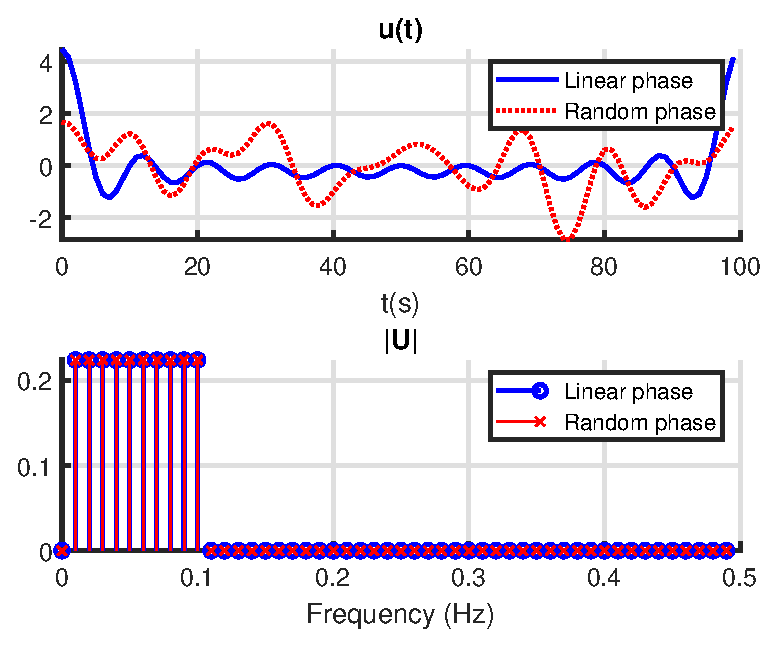
\includegraphics[width = 0.65\textwidth]{figures/MS_u0_u.eps}
    \caption{Comparison between a linear phase multisine and a random phase multisine with the same RMS value.}
    \label{fig:linear_random_MS_compare}
\end{figure}

\newpage
\paragraph{Example}
Consider a DT system.
\begin{equation}
    G(z^{-1}) = \frac{0.4097 z^{-1} + 0.407 z^{-2}}{1 - 1.165 z^{-1} + 0.9813 z^{-2}}
    \label{eq:Gz_example}
\end{equation}
This system is excited by the random phase multisine shown in figure \ref{fig:MS_u}. The normalized frequency is the frequency divided by the sampling frequency. 0.5 represents the Nyquist frequency $f_s/2$. The steady state output of this system is shown in figure \ref{fig:MS_y}. Then the FRF can be calculated by using (\ref{eq:G=Y/U_MS}) at the excited frequencies. The actual FRF and calculated FRF are plotted in figure \ref{fig:MS_G}.

\begin{figure}[H]
    \centering
    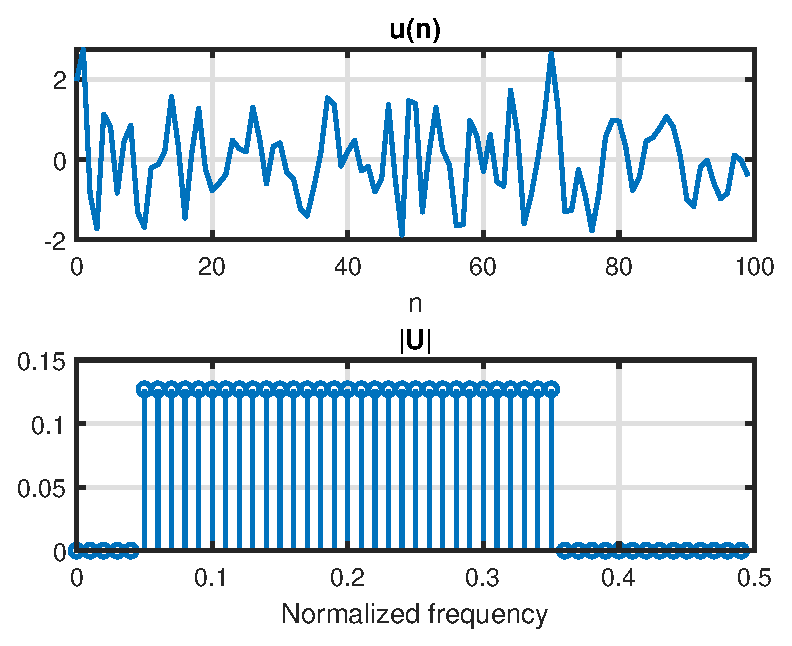
\includegraphics[width=0.65\textwidth]{figures/MS_u.eps}
    \caption{Input of the second-order system. Random phase multisine.}
    \label{fig:MS_u}
\end{figure}

\begin{figure}[H]
    \centering
    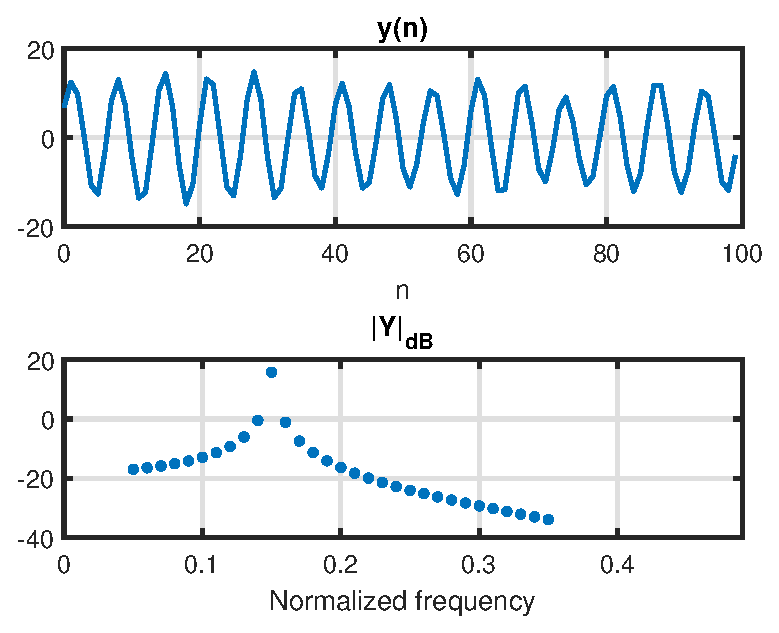
\includegraphics[width=0.65\textwidth]{figures/MS_y.eps}
    \caption{Output of the second-order system.}
    \label{fig:MS_y}
\end{figure}

\begin{figure}[H]
    \centering
    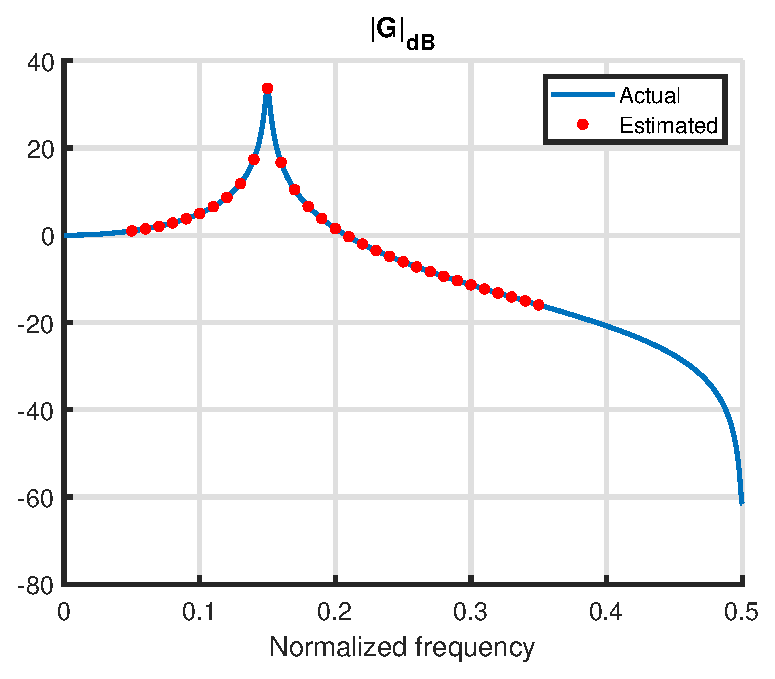
\includegraphics[width=0.65\textwidth]{figures/MS_G.eps}
    \caption{Magnitude FRF of the second-order system and the estimated FRF at the excited frequencies using (\ref{eq:G=Y/U_MS}).}
    \label{fig:MS_G}
\end{figure}

\newpage
\section{Measurement set-ups}
\subsection{Zero-order hold set-up}
In a lot of measurement set-ups, the input signal is generated digitally with a Zero-order hold (ZOH). This means that the signal is kept constant for a whole sampling period. At the sampling instants, a CT system $G(s)$ preceded by a ZOH can be modelled exactly as a DT system. \cite[eq. (34)]{ZOH_reference}
\begin{equation}
    G_{\mathrm{ZOH}}(z) = (1-z^{-1})  \mathcal{Z}\Big\{\mathcal{L}^{-1}\big\{\frac{G(s)}{s} \big\}\rvert_{t=n T_s}\Big\}
    \label{eq:ZOH_transform}
\end{equation}

The ZOH measurement set-up is shown in figure \ref{fig:zoh_setup}. In this case, the actuator $G_\mathrm{act}(s)$ is part of the FRF that is measured. The dynamics of the measurement device $G_y(s)$ must be calibrated perfectly ($G_y(s)=1)$ if one wants to measure the FRF from generator to output. Note that, in theory, the ZOH set-up is not allowed to contain anti-alias filters.
\begin{figure}[H]
    \centering
    \includegraphics[width =0.65\textwidth]{figures/ZOH_setup.png}
    \caption{Zero-order hold measurement set-up. \textcolor{red}{Red} indicates which parts are modelled. Taken from \cite{identification_of_dynamical_sytems_slides}.}
    \label{fig:zoh_setup}
\end{figure}
Thus, if no anti-alias filter is used at the output and assuming that the actuator is perfect $G_{\textrm{act}}(s)=1$, when a CT system is excited with a ZOH and is sampled, we are actually measuring the ZOH version of the FRF and not the CT FRF directly. This is bad news if we want to measure the CT FRF $G(s)$. However, this can be circumvented. When $|f| \ll f_s/2$, there isn't a big difference between the CT FRF $G(s)$ and the ZOH version of $G(s)$.
\begin{equation}
    G(j 2 \pi f) \approx G_{\mathrm{ZOH}}(e^{j 2 \pi f T_s})
    \label{eq:Gzohapprox}
\end{equation}

So, when the goal is to measure a CT FRF with a ZOH set-up, care must be taken to stay within the region where this approximation holds. This can be accomplished by making sure that the highest excited frequency in the input signal is well below the sampling frequency of the measurement set-up.
\begin{equation*}
    f_{\text{max}} \ll f_s/2
\end{equation*}

\paragraph{Example}
Consider a second order system.
\begin{equation*}
    G(s) = \frac{\omega_0^2}{s^2 + 2 \zeta \omega_0 s + \omega_0^2} \text{ with } \omega_0 = 2 \pi 0.3 [\text{rad}/s] \text{ and } \zeta = 0.01
\end{equation*}
Applying the ZOH transformation (\ref{eq:ZOH_transform}) to this system with $f_s = 2 \text{Hz}$ results in the DT system that was used in previous examples (\ref{eq:Gz_example}). The magnitude FRF of both the CT system and the ZOH version of it are plotted in figure \ref{fig:Gzoh_example}. Notice that the DT system has a periodic FRF while the CT system does not. Moreover, at the low frequencies, both FRFs overlap. The approximation (\ref{eq:Gzohapprox}) is worse once the frequency gets close to $f_s/2$.

\begin{figure}[H]
    \centering
    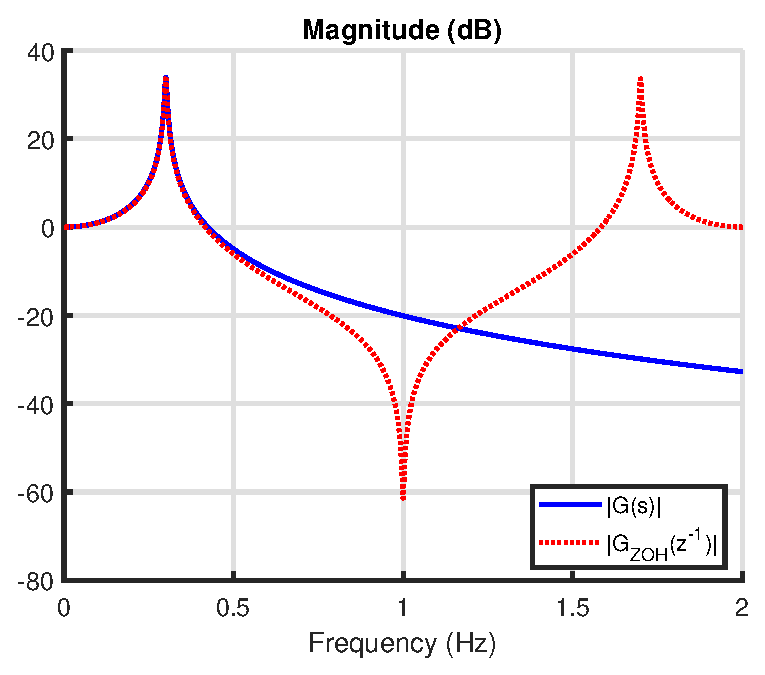
\includegraphics[width=0.65\textwidth]{figures/ZOH.eps}
    \caption{Magnitude FRF of the second-order system and the magnitude FRF of the ZOH version of it with $f_s = 2 \text{Hz}$.}
    \label{fig:Gzoh_example}
\end{figure}

\subsection{Band-limited set-up}
\label{sec:band-limited}
Even if one uses a high sampling frequency $f_s$, the actuator dynamics will still influence the measurement of the FRF when using a ZOH set-up. This is not an issue when a band-limited set-up is used. The band-limited set-up is shown in figure \ref{fig:BL_setup}. In a band-limited set-up, the input to the system can still be generated by a ZOH. But the input to the system must be measured and an anti-alias filter must be used to avoid aliasing. By measuring the input to the system, the dynamics of the actuator won't be part of the FRF estimate. The output of the system must also go through an anti-alias filter before being measured. A relative calibration is needed if one wants to measure the FRF from the input to the output. Concretely this means that the ratio of the anti-alias filters $G_y(s)/G_u(s)$ must be taken into account when processing the measurements.

\begin{figure}[H]
    \centering
    \includegraphics[width =0.65\textwidth]{figures/BL_setup.png}
    \caption{Band-limited measurement set-up. \textcolor{red}{Red} indicates which parts are modelled. Taken from \cite{identification_of_dynamical_sytems_slides}.}
    \label{fig:BL_setup}
\end{figure}


\section{System transients}
\label{sec:system_transients}
The first condition of perfect reconstructability (periodicity) implies that the signal has been repeating forever until now and will repeat forever in the future. This is not realistic; when a system is excited, the excitation must have started at some time in the past and must end at some point in the future. In the example of the previous section we had briefly mentioned that the measurements were taken in steady state. Concretely, the input was applied to the system for 20 periods and only the last period was used for the analysis, thereby ensuring that the system transients have faded away. This can be quantified by calculating the RMS of the difference between the output of the $p$-th period and the output of the last period. This is plotted in figure \ref{fig:MS_transients_RMS_error}. The RMS of the difference decreases exponentially. If the measurements were noisy, the RMS of the difference would decrease until the transients are below noise level, at which point the transients can be said to have faded away. In this case, the RMS of the difference reaches approximately $10^{-7}$ by the 20-th period, which is negligible for our purposes.

\begin{figure}[H]
    \centering
    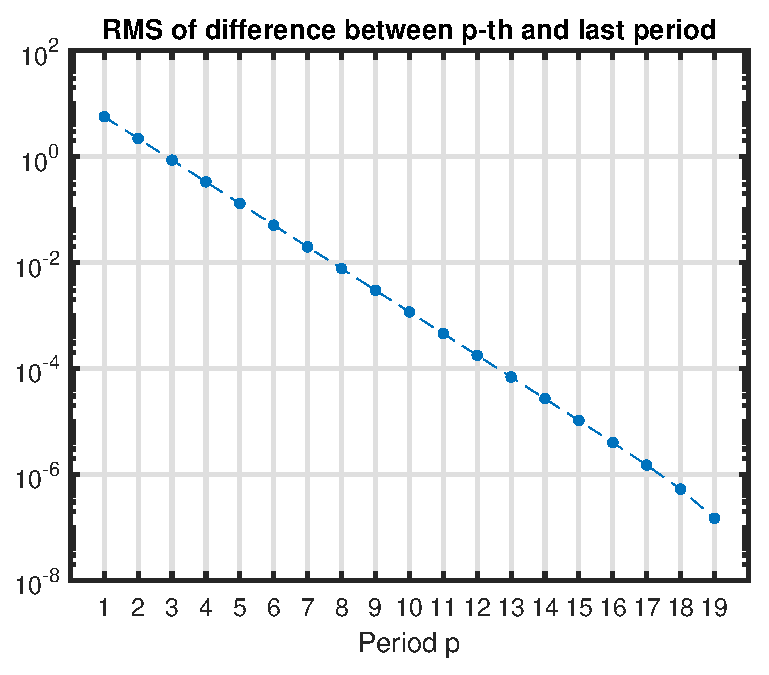
\includegraphics[width=0.65\textwidth]{figures/MS_transients_RMS_error.eps}
    \caption{RMS of the difference between the output of every period and the output of the last period.}
    \label{fig:MS_transients_RMS_error}
\end{figure}

It turns out that the transient term is just a rational function added on top of the steady state output spectrum.
\begin{equation}
\boxed{
    Y(k) = G(e^{-j 2 \pi k/N}) U(k) + T(k)
    }
    \label{eq:Y=GU+T}
\end{equation}
with
\begin{equation*}
    T(k) = \frac{I(e^{-j 2 \pi k/N})}{A(e^{-j 2 \pi k/N})}
\end{equation*}

$I(e^{-j 2 \pi k/N})$ is a polynomial in $e^{-j 2 \pi k/N}$ whose coefficients depend on the difference between samples from the previous period and samples from the current period. This is proven for DT systems in appendix \ref{appendix:transient_term}. The transient term for CT systems will be discussed afterwards.


If $u(n)$ and $y(n)$ are periodic, then $T(k)=0$, because $I(e^{-j 2 \pi k/N})$ only depends on the difference between the in- and output at the end of the current period and the in- and output at the end of the previous period. In this case (\ref{eq:Y=GU+T}) simplifies to what we had before.
\begin{equation*}
    Y(k) = G(e^{-j 2 \pi k/N}) U(k)
\end{equation*}

A key property of the transient term $T(k)$ is that it is a ``smooth'' function of the frequency $k$. This is due to the fact that it is a rational form of $e^{-j2\pi k/N}$. This property can be used to suppress the transient, as will be explained later. Another property of $T(k)$ is that its denominator is the same as the denominator of $G(e^{-j 2 \pi k/N})$. Therefore, the transient term will ``resemble'' the shape of the FRF.

\paragraph{CT transients}
Similar results can be derived for CT systems \cite{pintelon_book}.
\begin{equation*}
\boxed{
    Y(k) = G(j\omega)U(k) + T(k) + \delta(k)
    }
\end{equation*}
In this case, the numerator of $T(k)$ depends on the difference in initial conditions at $t=0$ and $t=T=n T_s$:
\begin{equation*}
    \Big[\frac{d^p y}{{dt}^p}(T) - \frac{d^p y}{{dt}^p}(0)\Big] \text{ and } \Big[\frac{d^p u}{{dt}^p}(T) - \frac{d^p u}{{dt}^p}(0)\Big]
\end{equation*}
with $p \in \mathds{N}$ and $p < \max{(n_a,n_b)}$, $n_a$ and $n_b$ being the order of the denominator and numerator of $G(s)$ respectively. An additional term $\delta(k)$ pops up. This is the alias error and it can be generated when the transient $T(j\omega)$ overextends into the aliasing frequencies  $f > f_s/2$. It is present even if the signals have been low-pass filtered. Because the alias error $\delta(k)$ is also smooth, it can be grouped together with the transient term $T(k)$.


\newpage
\paragraph{Example}
Again, the same second-order system (\ref{eq:Gz_example}) of the previous section is used. This time we will take a look at the estimation error.
\begin{align*}
    G_{\mathrm{est}}(e^{-j 2 \pi k/N}) - G(e^{-j 2 \pi k/N}) &= \frac{Y(k)}{U(k)} - G(e^{-j 2 \pi k/N}) \\ &=  \frac{G(e^{-j 2 \pi k/N}) U(k) + T(k)}{U(k)} - G(e^{-j 2 \pi k/N}) \\ &=  \frac{T(k)}{U(k)}
\end{align*}
As the magnitude spectrum of $u(n)$ is flat, the magnitude of the estimation error will be proportional to the magnitude of the transient term.

The estimation error for the FRF estimated from the first and 20th period is shown in figure \ref{fig:MS_G_transients}. The error of the FRF calculated from the last period is around $-150 \text{dB}$, which is negligible. In other words, there is no transient term as the system is in steady state. The error for the first period is a smooth function of the frequency and ``resembles'' the shape of the transfer function as expected.

\begin{figure}[H]
    \centering
    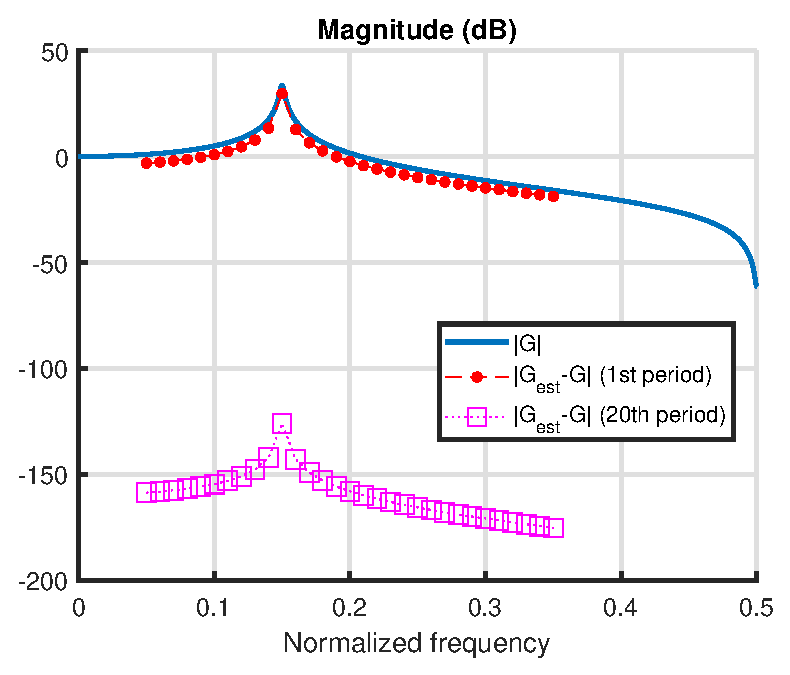
\includegraphics[width=0.65\textwidth]{figures/MS_G_transients.eps}
    \caption{Magnitude FRF of the second-order system and the estimation errors of the FRF at the excited frequencies using (\ref{eq:G=Y/U_MS}) for the data from the first period and the 20th period.}
    \label{fig:MS_G_transients}
\end{figure}

\section{Frequency domain methods}
Till now we have been treating CT and DT systems as separate cases. However, FD methods can be generalized to both CT and DT systems. There is no reason why a FD method should only work for one and not the other. To generalize these methods it is useful to define $\Omega$ to encompass both CT and DT models. $\Omega$ can either be $s$ or $z^{-1}$.
\begin{equation*}
    \Omega = \begin{cases}
        s & \text{if working in continuous-time (CT)} \\
        z^{-1} & \text{if working in discrete-time (DT)} 
    \end{cases}
\end{equation*}
Thus, denoting an LTI system as $G(\Omega)$ is not specific to CT or DT systems. When the FRF is evaluated in the DFT frequencies $\omega_k = 2 \pi k f_s/N$ it, is denoted $\Omega_k$.
\begin{equation*}
    \Omega_k = \begin{cases}
        j \omega_k = j 2 \pi k f_s/N& \text{if working in continuous-time (CT)} \\
        e^{-j \omega_k T_s} = e^{-j 2 \pi k/N} & \text{if working in discrete-time (DT)} 
    \end{cases}
\end{equation*}

\section{White noise}
\label{sec:white_noise}
White noise is a random signal with a flat power spectrum. A zero-mean Gaussian sequence is white noise.
\begin{equation*}
    v(n) \sim \mathcal{N}(0,\sigma^2)
\end{equation*}
Let's assume that a measurement is perturbed by this white noise.
\begin{equation*}
    x(n) = x_0(n) + v(n)
\end{equation*}
Due to the linearity of the DFT one obtains
\begin{equation*}
    X(k) = X_0(k) + V(k)
\end{equation*}
Thus it is interesting to understand the properties of the DFT of this white noise sequence.
\begin{equation*}
    V(k) = \frac{1}{N}\sum_{n=0}^{N-1} v(n) e^{-j 2\pi k n/N}
\end{equation*}
It turns out that (see appendix \ref{appendix:white_noise})
\begin{align*}
    &\mathbb{E}\{V(k)\} = 0\\
    &\mathbb{E}\{|V(k)|^2\} = \frac{1}{N} \sigma^2 \\
    &\mathbb{E}\{V^2(k)\} = 0 \text{ if mod}(2k,N) \neq 0
\end{align*}

\section{Periodic signals}
What happens to the DFT spectrum when we apply a signal periodically? Let's assume that we have a sequence $\tilde{x}(n)$ of length $N$ with corresponding DFT
\begin{equation*}
    \tilde{X}(k) = \sum_{n=0}^{N-1} \tilde{x}(n) e^{-j 2\pi k n/N}
\end{equation*}
Now, the sequence $\tilde{x}(n)$ will be repeated one more time to obtain a sequence of length $2N$.
\begin{equation*}
    x(n) = \begin{cases}
        \tilde{x}(n) &\text{ if } 0 \leq n < N - 1\\
        \tilde{x}(n-N) &\text{ if } N \leq n < 2N - 1
    \end{cases}
\end{equation*}
The DFT of $x(n)$ is then given by
\begin{align*}
    X(k) &= \frac{1}{2N}\sum_{n=0}^{2 N-1} \tilde{x}(n) e^{-j 2\pi k n/(2N)} = \frac{1}{2N}\sum_{n=0}^{N-1} \tilde{x}(n) e^{-j 2\pi k n/(2N)} + \frac{1}{2N}\sum_{n=N}^{2N-1} \tilde{x}(n-N) e^{-j 2\pi k n/(2N)} \\
    &= \frac{1}{2N}\sum_{n=0}^{N-1} \tilde{x}(n) e^{-j 2\pi k n/(2N)} + \frac{1}{2N}\sum_{n=0}^{N-1} \tilde{x}(n) e^{-j 2\pi k n/(2N)}  e^{-j 2\pi k/2} \\
    &= \frac{1}{N}\sum_{n=0}^{N-1} \tilde{x}(n) e^{-j 2\pi k n/(2N)} \frac{1+e^{-j 2\pi k/2}}{2}
    \end{align*}
Evaluating this in $2k$ and $2k+1$ gives
\begin{align*}
    &X(2k) = \tilde{X}(k)\\
    &X(2k+1) = 0
\end{align*}
Thus, the even DFT lines will contain the information of $X(k)$ and the odd DFT lines will be zero.

This result can be generalized to a signal that is repeated $P$ times.
\begin{equation*}
\boxed{
    %x(n) = \tilde{x}(\text{mod}(n,P)) \Rightarrow 
    X(kP+r) =
    \begin{cases}
        \tilde{X}(k) &\text{ if } r = 0\\
        0 & \text{ if } r = 1,\ldots,P-1\\
    \end{cases}
}
\end{equation*}

\newpage
\paragraph{Example}
A random phase multisine ($N=40$) is created where the 3 lowest DFT bins are excited with an RMS value of 1. This signal is repeated $P=3$ times. The repeated signal is plotted in the TD and the FD in figure \ref{fig:periodic_MS}. It can be seen that in the periodic signal there are $P-1 = 2$ non-excited lines in between the excited lines.

\begin{figure}[H]
    \centering
    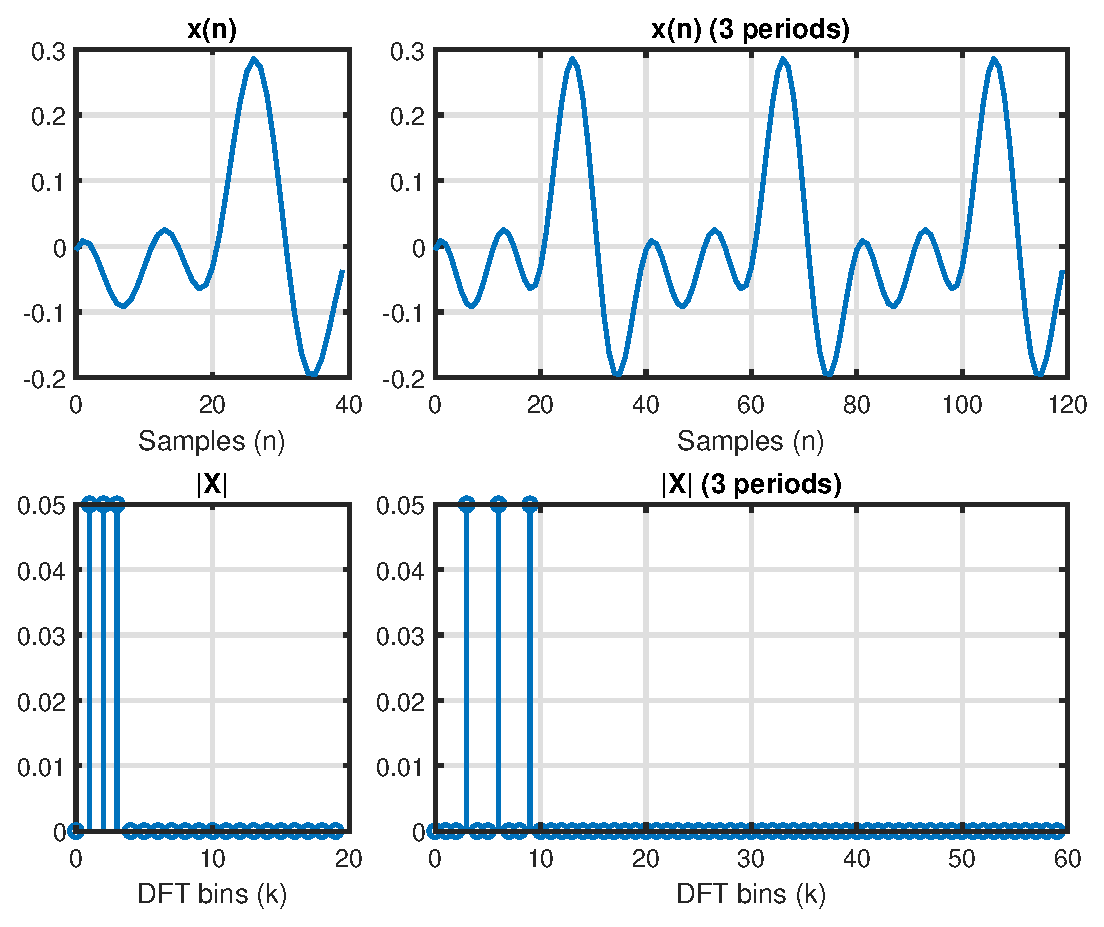
\includegraphics[width = 0.65\textwidth]{figures/periodic.eps}
    \caption{A multisine is repeated 3 times.}
    \label{fig:periodic_MS}
\end{figure}


\section{Transient suppression}
In section \ref{sec:system_transients} it was shown that transients in the output will negatively impact the quality of the FRF estimate. However, there are multiple ways to suppress these transients. The most obvious way is to wait for the system to enter steady state and to only start measuring once the transients have faded away. This is exactly what was done in the example of section \ref{sec:system_transients} (see figure \ref{fig:MS_G_transients}). There are also ways to suppress the transient without throwing away the measurements that are not in steady state. 3 of them will be discussed:
\begin{itemize}
    \item Windowing
    \item Parametric estimation
    \item The local polynomial method
\end{itemize}

\newpage
\subsection{Windowing}
There are many possible windows that one can choose from. The Hann window is a popular one.
\begin{equation}
    w(n) = \frac{1}{2} [1 - \cos(\frac{2\pi n}{N})] \,,\quad n = 0,\ldots,N-1
\end{equation}
The windowed input and output are then given by
\begin{equation*}
    u_w(n) = w(n) u(n) \text{ and } y_w(n) = w(n) y(n)
\end{equation*}
A multiplication in the TD becomes a convolution in the FD.
\begin{equation*}
    U_W(k) = W(k) * U(k) \text{ and } Y_W(k) = W(k) * Y(k) 
\end{equation*}
with $W(k) = \frac{1}{2} \delta(k) - \frac{1}{4} \delta(k+1) - \frac{1}{4} \delta(k-1)$.
The windowed estimate of the FRF is then given by
\begin{equation}
    G_W(\Omega_k) = \frac{Y_W(k)}{U_W(k)}
    \label{eq:G_W}
\end{equation}

Let's now see why windowing will reduce the effect of the transient.
\begin{equation*}
    Y_W(k) = W(k) * (G(\Omega_k) U(k) + T(k))
\end{equation*}
For the first term the following approximation can be made:
\begin{equation*}
    W(k) * [G(\Omega_k) U(k)] \approx G(\omega_k) [W(k) * U(k)] = G(\omega_k) U_W(k)
\end{equation*}
Hereby it is assumed that $G(\Omega_{k-1}) \approx G(\Omega_{k}) \approx G(\Omega_{k+1})$. In other words, $G(\Omega)$ is flat around $\Omega_k$. (\ref{eq:G_W}) then becomes
\begin{equation*}
    G_W(\Omega_k) \approx G(\Omega_k) + \frac{T_W(k)}{U_W(k)}
\end{equation*}
The trick now is to use the property that $T(k)$ is a smooth function of the frequency. Let's assume that $T(k)$ can be captured locally by a second order polynomial.
\begin{equation*}
    T(k) = a k^2 + b k + c
\end{equation*}
Windowing $T(k)$ gives
\begin{equation*}
    T_W(k) \propto 2 T(k) - T(k+1) - T(k-1) = - 2 a
\end{equation*}
This is a bit like taking the second order derivative, which suppresses the transient.

\newpage
\paragraph{Example}
The DT system (\ref{eq:Gz_example}) is taken again. The same input as in figure \ref{fig:MS_u} is used. The estimation error of the FRF with and without windowing is shown in figure \ref{fig:hann_window_FRF}. Windowing gives better results, except near the resonance frequency. This is because the approximation that $G(\Omega)$ is flat does not hold in this region.
\begin{figure}[H]
    \centering
    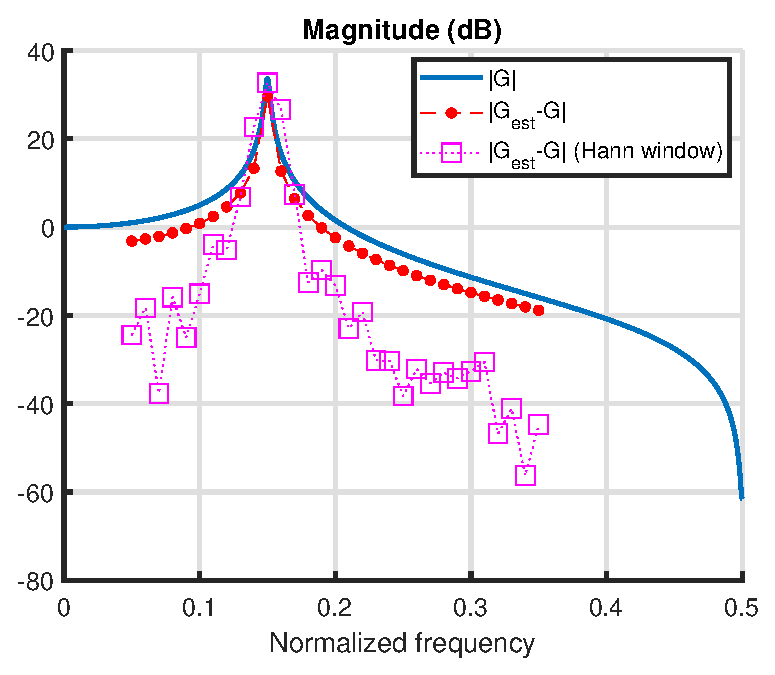
\includegraphics[width =0.65 \textwidth]{figures/hann_window.eps}
    \caption{Comparison of FRF estimation error without and with Hann windowing.}
    \label{fig:hann_window_FRF}
\end{figure}


\subsection{Parametric estimation}
Till now, only nonparametric estimates of the FRF were discussed. Unlike line-fitting, where one is interested in the slope and offset of the line, the nonparametric estimate does no such thing. The result of the nonparametric estimate is the FRF estimate at every excited frequency. However, in a sense there are still parameters: these are the FRF estimates at every frequency bin $k \in \kexc$.

The TF of the system is however still given by a rational function. The coefficients of this rational function can be estimated. The transient term is also a rational function and the parameters describing it can also be included in the estimation.
\begin{equation*}
    Y(k) = G(\Omega_k) U(k) + T(k)
\end{equation*}
Using $G(\Omega_k) = \frac{B(\Omega_k)}{A(\Omega_k)}$ and $T(k) = \frac{I(\Omega_k)}{A(\Omega_k)}$ the expression above can be rewritten as
\begin{equation}
    A(\Omega_k) Y(k) - B(\Omega_k) U(k) - I(\Omega_k) = 0
    \label{eq:AY-BU-I=0}
\end{equation}
$A(\Omega_k)$ is a polynomial of order $n_a$ and $B(\Omega_k)$ is a polynomial of order $n_b$. (\ref{eq:I_explicit}) in appendix \ref{appendix:transient_term} is an explicit formula for $I(\Omega_k)$. From this formula, it can be verified that $I(\Omega_k)$ is a polynomial of order $n_I$ with
\begin{equation*}
    n_I = \max{(n_a,n_b)}-1
\end{equation*}
For CT systems, there is also an alias error on top of the transient term. These errors can also be captured well by a polynomial. Grouping the alias error together with the $I(\Omega_k)$ results in \cite[Section 6.3.2.3]{pintelon_book}
\begin{equation*}
    n_I \geq \max{(n_a,n_b)}
\end{equation*}
After a bit of calculations, (\ref{eq:AY-BU-I=0}) can be turned into
\begin{equation*}
    \begin{bmatrix}
    \vdots & & \vdots & \vdots & & \vdots & \vdots & & \vdots \\
    Y(k) & \hdots & Y(k) \Omega_k^{n_a} & 
    U(k) & \hdots & U(k) \Omega_k^{n_b} & 
    1    & \hdots &      \Omega_k^{n_I} \\
    \vdots & & \vdots & \vdots & & \vdots & \vdots &  & \vdots
    \end{bmatrix}
    \begin{bmatrix}
    a_0 \\ \vdots \\ a_{n_a} \\ 
    -b_0 \\ \vdots \\ -b_{n_b} \\
    -i_0 \\ \vdots \\ -i_{n_I}
    \end{bmatrix} = 0
\end{equation*}
This can be solved by calculating the right null-space of the first matrix. The coefficients $i_p$ will capture the transient. Note that the null space is empty if the measurements are noisy. We won't go into these details in this work, so the interested reader is referred to \cite{markovsky_book}.

\paragraph{Example}
Again, the DT system (\ref{eq:Gz_example}) is used with the same input shown in figure \ref{fig:MS_u}. The parameters are determined as described above. The resulting FRF estimation error is plotted in figure \ref{fig:transient_parametric}. Note that as a parametric representation is obtained, the FRF can be calculated at all frequencies. The error is around $-300 \text{dB}$, which is MATLAB's precision. This means that the error is negligible and that the transient has been fully suppressed.

\begin{figure}[H]
    \centering
    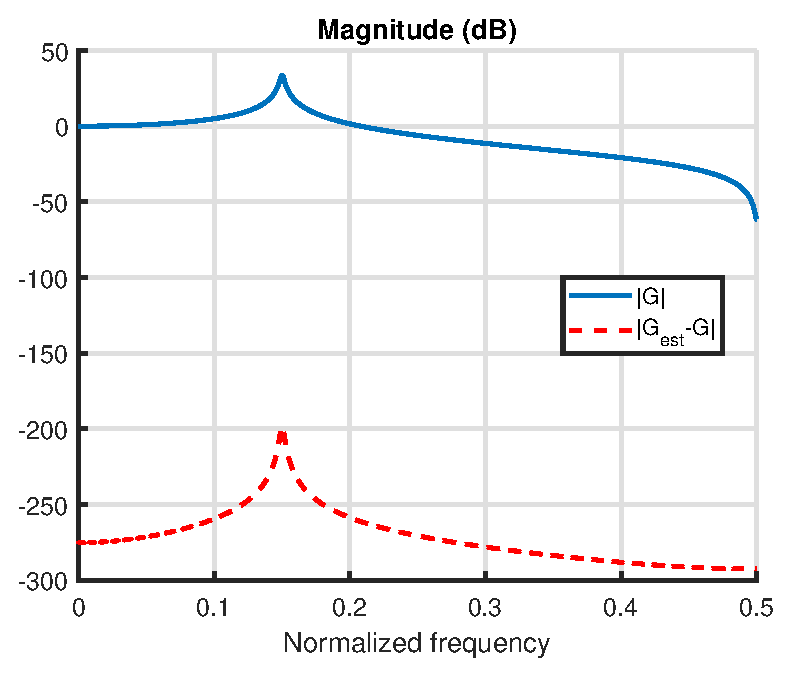
\includegraphics[width=0.65\textwidth]{figures/parametric_transient.eps}
    \caption{FRF estimation error for the parametric estimation of the TF with transient terms.}
    \label{fig:transient_parametric}
\end{figure}


\section{Local polynomial method}
\label{sec:LPM}
The idea of the local polynomial method (LPM) is quite simple. There are multiple variants of the LPM, but here we will focus on the robust LPM for periodic excitations. More information about all the variants of the LPM can be found in \cite[Chapter 7]{pintelon_book}.

\subsection{Response of a system excited by a periodic input}
For the robust LPM for periodic signals to work, at least $P=2$ periods must be measured. Let's assume for the sake of simplicity that the input $\tilde{u}(n)$ is noiseless and in steady state. $\tilde{u}(n)$ is applied $P$ consecutive times to the system.
%\begin{equation*}
%    u(n) = \tilde{u}(\text{mod}(n,P)) \,,\quad n = 0,1,\ldots,N P-1
%\end{equation*}
The spectrum of the input $u(n)$ is
\begin{equation}
    U(kP+r) =  
    \begin{cases}
        \tilde{U}(k) &\text{ if } r = 0\\
        0 & \text{ if } r = 1,\ldots,P-1
    \end{cases}
    \label{eq:U(kP+r)}
\end{equation}
It will resemble the spectrum shown in figure \ref{fig:periodic_MS}. Assuming that the output is perturbed by additive noise, the output spectrum is given by
\begin{equation*}
    Y(kP+r) = G(kP+r)U(kP+r) + T(kP+r) + N_y(kP+r)
\end{equation*}
$T(kP+r)$ is the transient term that arises from the fact that the system might not be in steady state. $N_y(kP+r)$ is additive noise that is added to the output. It can either be white noise (see section \ref{sec:white_noise}) or filtered white noise. Using (\ref{eq:U(kP+r)}), we can be more specific about the output spectrum.
\begin{equation*}
\boxed{
    Y(kP+r) =
    \begin{cases}
     G(kP)U(kP) + T(kP) + N_Y(kP) &\text{ if } r = 0\\
     T(kP+r) + N_Y(kP+r) &\text{ if } r = 1,\ldots,P-1
     \end{cases}
     }
\end{equation*}

\paragraph{Example}
The system (\ref{eq:Gz_example}) is excited with the signal shown in figure \ref{fig:periodic_MS}. The output is perturbed by Gaussian white noise with a standard deviation of 0.005. The input and output spectra are plotted in figure \ref{fig:periodic_output}. The output spectrum at the DFT lines 3, 6 and 9 are dominated by the $G(kP)U(kP)$ term. There is a peak around the 18-th DFT line that corresponds to the transient term $T$. The 18-th DFT line corresponds to the normalized frequency $18/(NP) = 18/120 = 0.15$, which corresponds to the normalized resonance frequency of the system (see figure \ref{fig:transient_parametric} for example). This is to be expected as the transient resembles the shape of the transfer function. Finally, after the 30-th DFT bin, the noise terms $N_Y$ dominate the output.

\begin{figure}[H]
    \centering
    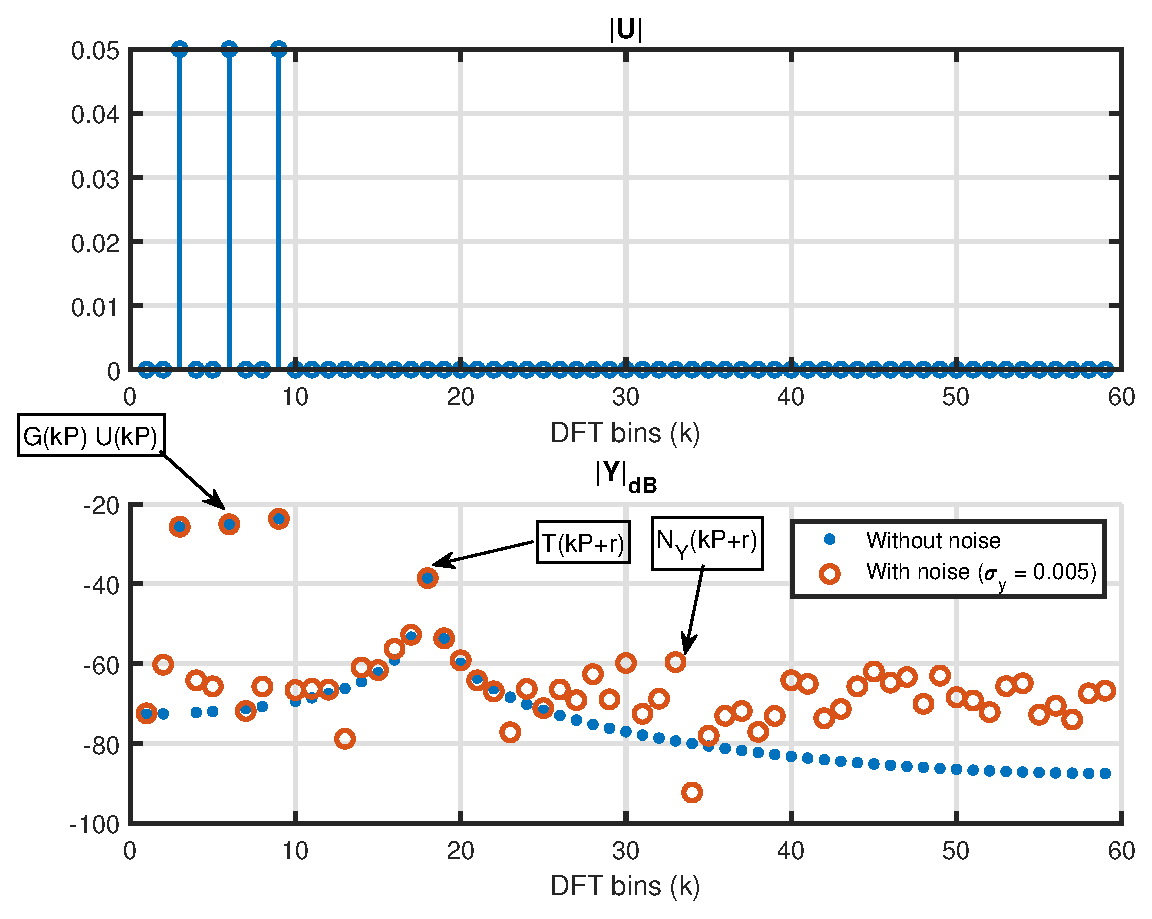
\includegraphics[width = 0.65\textwidth]{figures/periodic_output.eps}
    \caption{Input and output of the DT system (\ref{eq:Gz_example})}
    \label{fig:periodic_output}
\end{figure}

\subsection{Algorithm} Now we can finally discuss the algorithm of the robust LPM. The idea is to estimate the contribution of the transient term at the excited frequencies using the data at the non-excited frequencies. To this end, we will work in a window around every excited DFT bin. In the case of the previous example, the excited bins are k = 1, 2 and 3. Two parameters must be chosen by the user. The first one is the window size $2n$. We must use $n$ unexcited bins before and after $kP$. 

\paragraph{Example}
$k = 3$, $P=3$, $n=4$. We are working in a window around $Y(kP) = Y(9)$. We must use 4 unexcited bins before and after 9.
\begin{equation*}
    Y(9+r_i) \text{ with } r_i = -5,-4,-2,-1,1,2,4,5
\end{equation*}
For every one of the unexcited lines the following holds
\begin{equation*}
    Y(kP+r_i) = T(kP+r_i) + N_Y(kP+r_i)
\end{equation*}
The transient term can be modelled as a polynomial of $r$. This is because the transient is a smooth function of the frequency. The order of the polynomial $R$ is the second parameter that the user can choose.
\begin{equation*}
    T(kP+r) \approx T(kP) + \sum_{s=1}^R t_s(k) r^s
\end{equation*}
We can then find the polynomial of best fit through the points $Y(kP+r_i)$

\paragraph{Example continued}
Putting all the $Y(9+r_i)$ into a vector and choosing $R=2$ gives
\begin{equation*}
    \begin{bmatrix}
    Y(4)\\Y(5)\\Y(7)\\Y(8)\\Y(10)\\Y(11)\\Y(13)\\Y(14)
    \end{bmatrix} = 
    \begin{bmatrix}
    1 & (-5) & (-5)^2 \\
    1 & (-4) & (-4)^2 \\
    1 & (-2) & (-2)^2 \\
    1 & (-1) & (-1)^2 \\
    1 & 1 & 1^2 \\
    1 & 2 & 2^2 \\
    1 & 4 & 4^2 \\
    1 & 5 & 5^2 \\
    \end{bmatrix}
    \begin{bmatrix}
    T(9) \\ t_1(3) \\ t_2(3)
    \end{bmatrix} + 
    \begin{bmatrix}
    N_Y(4)\\N_Y(5)\\N_Y(7)\\N_Y(8)\\N_Y(10)\\N_Y(11)\\N_Y(13)\\N_Y(14)
    \end{bmatrix}
    \longrightarrow
    Y_n = K_n \Theta + V_n
\end{equation*}
The least squares solution is given by\footnote{Note that calculating the solution like this results in an ill-conditioned problem. The \textbackslash \ operator in MATLAB solves this problem using QR-factorisation, which is better conditioned. ($\theta = K_n \backslash Y_n$)}
\begin{equation*}
    \hat{\Theta} = (K_n^H K_n)^{-1}K_n^H Y_n
\end{equation*}
This results in an estimation of the transient term at the excited DFT bin $\hat{T}(9)$. The other terms $t_1(3)$ and $t_2(3)$ are not important.

Finally, the estimated transient term can be removed from the output spectrum at the excited DFT line.
\begin{equation*}
\boxed{
    \hat{Y}(kP) = Y(kP) - \hat{T}(kP)
}
\end{equation*}
Thus, the transient has been suppressed. The FRF can then be calculated simply as
\begin{equation*}
    \hat G(\Omega_k) = \frac{\hat{Y}(kP)}{U(kP)}
\end{equation*}
The entire procedure outlined here must be repeated for all $k \in \kexc$.

\subsection{Variance estimate}
Having a variance estimate of the output spectrum is useful for providing uncertainty bounds. It can also be used as a nonparametric weighting in parametric identification of the system transfer function. %\cite[Introduction]{nonparametric_periodic}

The residual is defined as the difference between the measured output spectrum and the predicted output spectrum.
\begin{equation*}
    \hat{V}_n = Y_n - K_n \hat{\Theta}
\end{equation*}
Assuming that the variance of the noise is white (flat) in the window $2n$, it can be used to estimate the variance at every $k \in \kexc$.
\begin{equation*}
    \hat\sigma^2_{\hat Y}(kP) = \frac{1}{q^{\text{noise}}} V_n^H V_n \,,\quad \text{ with } q^{\text{noise}} = 2 n - (R + 1) \text{ (degrees of freedom)}
\end{equation*}
A proof of this is given in appendix \ref{appendix:cov_est} and is based on \cite[Appendix 7.B]{pintelon_book}. The reason why we must divide by the degrees of freedom $q^{\text{noise}}$ and not by $2n$ is because $R+1$ parameters are estimated. This is analogous to the reason why the unbiased sample variance is calculated by dividing by the number of observations minus 1 when the population mean is also estimated. 

As $\hat G(\Omega_k) = \hat{Y}(kP)/U(kP)$, the variance of the FRF can be calculated as
\begin{equation}
    \hat\sigma^2_{\hat G}(\Omega_k) = \frac{\hat\sigma^2_Y(kP)}{|U(kP)|^2}
    \label{eq:variance_estimate_no_input_noise}
\end{equation}

\newpage
\subsection{Example}
The robust LPM is applied to measurements from the system (\ref{eq:Gz_example}). This time $N = 16384$ and $P=2$. The first $F=5000$ frequencies are excited with a random phase multisine with an RMS value 1. White Gaussian noise is added to the output with $\sigma_y = 0.2$. This corresponds to a signal-to-noise ratio (SNR) of $29.5 \mathrm{dB}$. This number is calculated as follows.
\begin{equation*}
    \mathrm{SNR}_{\mathrm{dB}} = 10 \log_{10} \Big ( \frac{\frac{1}{NP}\sum_{t=0}^{NP-1}y_0(t)^2}{\sigma_y^2} \Big ) = 29.5 \mathrm{dB}
\end{equation*}
The numerator is the mean of the squares of the noiseless output $y_0$ and the denominator is the power of the noise. The SNR is quite high as a consequence of the resonance that is present in the transfer function. 100 noise realizations are simulated while keeping the same random phase multisine as an input and the root-mean square (RMS) error is calculated to get an idea of the effectiveness of the estimator.
\begin{equation*}
    \text{RMS}[|\hat G - G|](\Omega_k) = \sqrt{\frac{1}{100}\sum_{i=1}^{100}|\hat G^{(i)}(\Omega_k)-G(\Omega_k)|^2} 
\end{equation*}
with $\hat G^{(i)}(\Omega_k)$ being the nonparametric estimate of $G(\Omega_k)$ for the $i$-th noise realization. The parameters used for the LPM are $R=2$, $n = 6$ which results in $q^{\text{noise}} = 9$ degrees of freedom. To make the results more presentable, the data points are taken together in windows of size 50 and are averaged. The results are shown in figure \ref{fig:LPM_example}. Not taking the transient into account is significantly worse around the resonance frequency of the system. The transient resembles the FRF of the system, which is why the error is most pronounced around the resonance frequency. However, far away from the resonance frequency, not taking the transient into account is approximately 1 dB better than using the Robust LPM. This is because the transient term is below the random noise contribution. LPM uses a noisy estimate of the transient and this estimate is subtracted from the output spectrum, leading to an increased variance. Finally, the robust LPM seems to be slightly better than windowing in this simulation.


\begin{figure}[H]
    \centering
    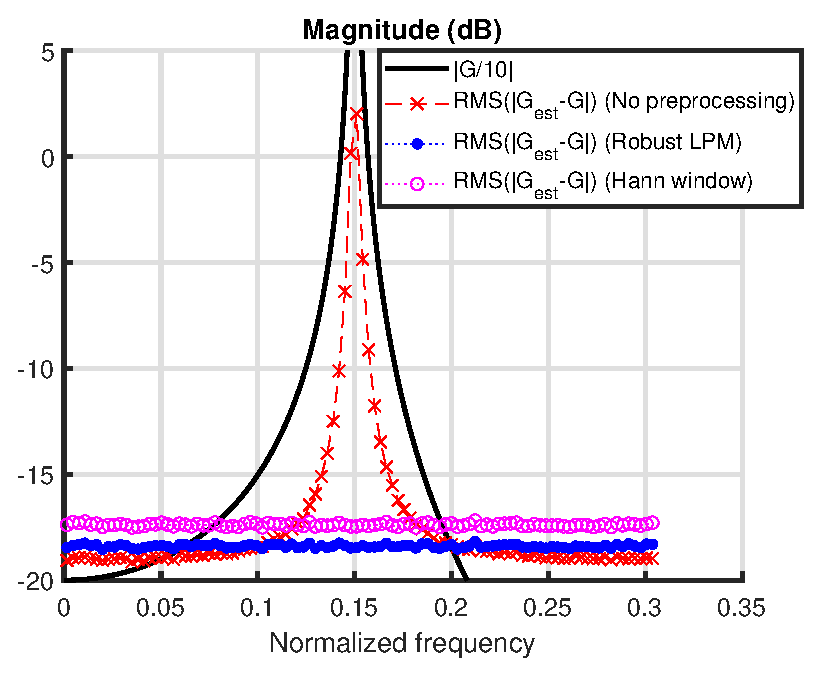
\includegraphics[width = 0.65\textwidth]{figures/LPM_example.eps}
    \caption{Comparison of the RMS error for the nonparametric estimate acquired without preprocessing, with windowing and with the robust LPM. $R=2$, $n = 6$, $q^{\text{noise}} = 9$.}
    \label{fig:LPM_example}
\end{figure}

\subsection{Choice of the order and degrees of freedom}
\label{sec:choice_order_dof}
Two parameters can be chosen by the user when performing the robust LPM analysis: the order of the polynomial approximation and the degrees of freedom used to estimate the noise variance.

\paragraph{Order}
A good way to choose the order is to start at $R=2$ and increment it in steps of two until the estimate of the variance $\hat \sigma^2_{\hat G}$ stops decreasing.

\paragraph{Degrees of freedom}
Increasing the degrees of freedom $q^{\text{noise}}$ will increase the window size $2n$. This gives a better estimation of the variance. There is a trade-off however: it was assumed that the noise variance is white (flat) in the window $2n$. Thus, making the window size too big will result in a loss of frequency resolution. Additionally, making the window size $2n$ bigger means that the transient is approximated by a polynomial over a larger window. At that point it might be necessary to increase the order $R$ of the polynomial.

\section{Generalization}
Many things were simplified until now. A few of the assumptions that were made are:
\begin{itemize}
    \item The input is noiseless.
    \item White Gaussian noise noise was simulated in the example, but what if the noise is filtered white noise?
    \item There is no feedback from output to input.
    \item The input is a multisine. What about random excitations?
\end{itemize}
Each of these points will be discussed briefly.

\subsection{Noisy input}
Of course, the measurement of the input can be noisy. Thankfully, the robust LPM is also able to estimate the input noise variance for periodic excitations. Given that the input is not known perfectly, the estimate of the FRF variance (\ref{eq:variance_estimate_no_input_noise}) is not correct any more. In general, the variance of an FRF estimate $\hat G(\Omega_k)$ can be approximated by
\begin{equation*}
    \hat \sigma_{\hat G}^2(k) = |\hat G(\Omega_k)|^2 \Bigg(\frac{\hat{\sigma}_{Y}^2(k)}{|\hat{Y}(k)|} + \frac{\hat{\sigma}_{U}^2(k)}{|\hat{U}(k)|}
-2\mathrm{Re}\left(\frac{\hat{\sigma}^2_{YU}(k)}{Y(k)\overline{U(k)}}\right) \Bigg)
\end{equation*}

The equation above is only applicable when the excitation is periodic and when the FRF is estimated by dividing the output spectrum $Y(k)$ by the input spectrum $U(k)$. It is also possible to estimate the variance of the noise for arbitrary excitations, but different formulas must be used \cite[Section 2.6]{pintelon_book}.

\subsection{Filtered white noise}
For simplicity sake, filtered white noise at the sampling instants is defined as
\begin{equation*}
    v(n) = S(z^{-1}) e(n) \,,\quad \text{ with } e(n) \sim \mathcal{N}(0,\sigma^2)
\end{equation*}
The power spectrum of this noise is not flat. This also means that the noise samples can be correlated over time.
\begin{equation*}
    \exists n,m \text{ with } n \neq m \text{ such that } \mathbb{E}\{v(n) v(m)\} \neq 0 
\end{equation*}
An important consequence of filtered white noise is that there will also be noise transients in the measurements.
\begin{equation*}
    V(k) = S(\Omega_k) E(k) + T_S(\Omega_k)
\end{equation*}
As the input of the noise filter is random, the noise transients will never fade away. This means that when one waits long enough for the system $G(\Omega)$ to enter steady state, there will still be noise transients in the measurements. This is where the LPM can also be useful.

\subsection{Feedback}
\label{sec:feedback}
Consider the measurement set-up shown in figure \ref{fig:neg_feedback_system}. An LTI system $G(z^{-1})$ is in negative feedback and the output is perturbed by process noise.

\begin{figure}[H]
    \centering
    \includegraphics[width = 0.65\textwidth]{figures/system.pdf}
    \caption{LTI system in negative feedback with additive process noise.}
    \label{fig:neg_feedback_system}
\end{figure}

The Z-transform of the output and input are given by
\begin{align*}
    &Y(z) = \frac{G}{1+G} R(z) + \frac{1}{1+G} V(z)\\
    &U(z) = \frac{1}{1+G} R(z) - \frac{1}{1+G} V(z)
\end{align*}
Noise that affects the output also affects the input due to the feedback. Two possibilities will be considered: $r(n)$ is a multisine and $r(n)$ is a random signal. Assuming that the process noise $v(n)$ is a Gaussian white noise sequence with variance $\sigma_v^2$ we get
\begin{equation*}
    \mathbb{E}\{V(k)\} = 0 \text{ and } \mathbb{E}\{|V(k)|^2\} = \sigma_v^2(k)/N
\end{equation*}

\paragraph{$\boldsymbol{r(n)}$ is a multisine}
In this case we can apply multiple periods $P$ to the system. It is assumed that enough time has passed for the system transient to fade away and the noise transients will be neglected.
\begin{align*}
    &Y^{(p)}(k) = \frac{G(\Omega_k)}{1+G(\Omega_k)} R^{(p)}(k) + \frac{1}{1+G(\Omega_k)} V^{(p)}(k)\\
    &U^{(p)}(k) = \frac{1}{1+G(\Omega_k)} R^{(p)}(k) - \frac{1}{1+G(\Omega_k)} V^{(p)}(k)
\end{align*}
The superscript $(p)$ denotes the period of the measurement. The nonparametric FRF can then be estimated with
\begin{equation}
    \hat G(\Omega_k) = \frac{ \frac{1}{P}\sum_{p=0}^P Y^{(p)}(k) } { \frac{1}{P}\sum_{p=0}^P U^{(p)}(k) }
    \label{eq:G_estimator_for_MS}
\end{equation}
Taking the limit for $P \rightarrow \infty$ will allow us to establish whether this estimator is consistent.
\begin{equation*}
    \lim_{P\rightarrow\infty} \hat G(\Omega_k) = \frac{ \mathbb{E}\{ Y^{(p)}(k) \}} { \mathbb{E}\{ U^{(p)}(k) \}} = G(\Omega_k)
\end{equation*}
The first equality applies the law of large numbers for independent experiments. And so this estimator is indeed consistent.

\paragraph{$\boldsymbol{r(n)}$ is an arbitrary signal}
For arbitrary signals it is not advised to use the estimator (\ref{eq:G_estimator_for_MS}) because a division by a small number is possible, resulting in an estimator that won't converge. Another thing that must be considered when working with arbitrary signals is that arbitrary signals are aperiodic. If we want to get a better estimate of the FRF we will need to cut the measurement into $M$ pieces of $N$ samples. If the total number of samples $N\!M$ is constant, this will results in a trade-off between the frequency resolution $f_s/N$ and noise suppression. An estimator that is used for arbitrary signals is
\begin{equation}
    \hat G(\Omega_k) = \frac{ \frac{1}{M}\sum_{m=0}^M Y^{(m)}(k) \overline{U^{(m)}(k)} } { \frac{1}{M}\sum_{m=0}^M U^{(m)}(k) \overline{U^{(m)}(k)} }
    \label{eq:G_estimator_for_random}
\end{equation}
Here there is no danger for the denominator to become small. This estimator is consistent when only the output is perturbed by noise. However, in our case the input is also perturbed. Taking the limit as $M \rightarrow \infty$ gives
\begin{equation*}
    \lim_{M\rightarrow\infty} \hat G(\Omega_k) = \frac{ \mathbb{E}\{ Y^{(m)}(k) \overline{U^{(m)}(k)}\}} { \mathbb{E}\{ U^{(m)}(k) \overline{U^{(m)}(k)} \}} = \frac{ S_{YU}(k)} { S_{UU}(k)}
\end{equation*}
with $S_{YU}$ being the cross-power spectrum between the output and input and $S_{UU}$ being the auto-power spectrum of the input. Assuming that the reference is zero-mean Gaussian white noise with variance $\sigma_r^2$ we get
\begin{equation*}
    \mathbb{E}\{R(k)\} = 0 \text{ and } \mathbb{E}\{|R(k)|^2\} = \sigma_r^2(k)/N
\end{equation*}
and the using fact that $R(k)$ and $V(k)$ are uncorrelated we get the following result
\begin{equation*}
    \lim_{P\rightarrow\infty} \hat G(\Omega_k) = \frac{G(\Omega_k) \sigma_r^2(k) - \sigma_v^2(k)}{\sigma_r^2(k) + \sigma_v^2(k)} \neq G(\Omega_k)
\end{equation*}
Thus, the estimator (\ref{eq:G_estimator_for_random}) is inconsistent.

\paragraph{Indirect method}
It is possible to get around the problem of the estimator (\ref{eq:G_estimator_for_random}) by also using the reference signal $r(n)$. Instead of modelling the transfer function from input $(u)$ to output $(y)$, we will model the transfer function from reference $(r)$ to output $(y)$ and from reference $(r)$ to input $(u)$.
\begin{equation}
    \hat G(\Omega_k) = \frac{ \frac{1}{P}\sum_{m=0}^P Y^{(m)}(k) \overline{R^{(m)}(k)} } { \frac{1}{P}\sum_{m=0}^P U^{(m)}(k) \overline{R^{(m)}(k)} }
    \label{eq:G_estimator_for_random_indirect}
\end{equation}
Doing some calculations brings us to
\begin{equation*}
    \lim_{M\rightarrow\infty} \hat G(\Omega_k) = \frac{ \mathbb{E}\{ Y^{(m)}(k) \overline{R^{(m)}(k)}\}} { \mathbb{E}\{ U^{(m)}(k) \overline{R^{(m)}(k)} \}} = \frac{ S_{Y\!R}(k)} { S_{U\!R}(k)} = G(\Omega_k)
\end{equation*}
Thus, by keeping the reference signal and using it, it is possible to get a consistent estimate when using arbitrary excitations.

\newpage
\section{Conclusion}
Multisines can be used to estimate the FRF nonparametrically. The robust LPM allows for the transients to be suppressed. Even if the system is in steady state, the noise transients can still deteriorate the quality of the FRF estimate. This is a reason why the robust LPM can be quite effective.

It is useful to keep the reference signal that is applied to the system. When the system is excited by an arbitrary excitation, this information can be used to get a consistent estimate of the FRF even if both the input and the output are perturbed by noise.

Finally, the authors of \cite{pintelon_book} offer MATLAB code that can perform the robust LPM for periodic and arbitrary excitations. These MATLAB function can also identify the best linear approximation of a nonlinear system. These functions can also handle MIMO systems.


